\documentclass[12pt, A4]{article}

\usepackage[utf8]{inputenc}
\usepackage{hyperref}
\usepackage[T1]{fontenc}
\usepackage{listings}
\usepackage[dvipsnames]{xcolor}
\usepackage{xparse}
\usepackage{graphicx}
\usepackage{changepage}
\usepackage{calc}

\title{\textbf{Odlagališče (clipboard)}}
\author{Simon Peter Goričar}
\date{\textsubscript{Ljubljana 2021/22}}

\renewcommand*\contentsname{Kazalo}

\NewDocumentCommand{\code}{v}{%
	\texttt{\textcolor{ForestGreen}{#1}}%
}

\begin{document}
	\begin{titlepage}
		\maketitle
	\end{titlepage}
	\pagebreak
	
	\tableofcontents
	\pagebreak
	
	
	\section{Uvod}	
	Odložišče je med prvimi koncepti, ki jih spoznamo ob začetku uporabe računalnika. Njegova uporaba sega vse od osnovnega kopiranja besedila znotraj ene aplikacije (npr. besedilnega urejevalnika ali spletnega brskalnika) pa do bolj naprednih in arhitekturno zapletenih operacij, kot so kopiranje fotografij. V nekaterih primerih gre celo za lastniške (ang. "proprietary") vsebine, katerih format je prepoznaven samo določeni aplikaciji (npr. kopiranje zvočnega posnetka z dodatnimi metapodatki, ki so lastni določenemu urejevalniku zvoka in nimajo pomena zunaj njega).
	
	\subsection{Osnove}
	V osnovi vsi odložiščni sistemi podpirajo vsaj naslednje akcije\textsuperscript{\cite{winclipboardabout}}:
	\begin{itemize}
		\item \textbf{Rezanje -} iz izvorne aplikacije se izbrana vsebina odstrani in shrani v odložišče. Način shrambe je odvisen od implementacije.
		\item \textbf{Kopiranje -} iz izvorne aplikacije deluje podobno kot rezanje, le da se vsebina ne odstrani, samo še dodatno shrani v odložišče.
		\item \textbf{Lepljenje -} v ciljno aplikacijo pomeni vzeti vsebino, ki se nahaja v odložišču, in jo ponavadi v ciljni aplikaciji vnesti na mesto, kjer se nahaja kazalec.
	\end{itemize}
	
	Seveda je implementacija zgornjih akcij poljubna, kar pomeni, da aplikaciji sploh ni treba imeti kazalca ali očitnega mesta za kopiranje ali lepljenje. Koncept izbora vsebine se prav tako razlikuje od aplikacije do aplikacije - besedilni urejevalnik ima kazalec, raziskovalec ima izbor datotek, itd. Kljub temu se močno priporoča\textsuperscript{\cite{winclipboardabout}}, da aplikacije režejo, kopirajo ali lepijo le, ko uporabnik to zahteva, in ne gledajo ali upravljajo odložišča brez uporabnikovega strinjanja.
	
	
	\subsection{Zgodovina v enem odstavku}
	Koncept rezanja in lepljenja je oblikoval Pentti Kanerva, ekspert za programsko opremo na Stanfordski univerzi. Prvič je bil uporabljen v sedemdesetih, ko se je Larry Tesler v podjetju Xerox PARC domislil uporabnega načina rezanja in vstavljanja besedila za besedilni urejevalnik, ki so ga razvijali v podjetju. V samih začetkih je uporabnik izbral besedilo, ki ga je želel izbrisati in pritisnil na tipko za brisanje. Če je pozneje ugotovil napako in želel pridobiti nazadnje izbrisano besedilo nazaj, je pritisnil \textit{Esc} na tipkovnici. Ta ukaz pa je prilepil besedilo ne na mesto izbrisa, ampak na trenutno lokacijo kazalca. Takšni so bili v osnovi začetki odložišča - pravzaprav je šlo za sistem razveljavljanja napak\textsuperscript{\cite{designingiteractions}}.
	
	
	\subsection{Arhitekturna vprašanja}
	Različni operacijski in okenski sistemi implementirajo sistem za hranjenje odložišča na različne načine, a so morali vsi pri oblikovanju sistema v grobem odgovoriti na večino sledečih arhitekturnih vprašanj:
	\begin{itemize}
		\item Kateri del operacijskega sistema upravlja z odložiščnim sistemom (operacijski sistem, okenski sistem, ...)?
		\item Ali mora proces imeti okno (ali platformi soroden koncept), da lahko upravlja z odložiščem?
		\item Ali se vsebina odložišča prenese v medpomnilnik že ob ukazu za kopiranje ali naravnost v ciljni proces šele ob lepljenju?
		\item Kakšen standard (če sploh) se vzpostavi za številne oblike vsebine v odložišču?
		\item Kje hraniti ali kako prenesti večje kopice podatkov?
		\item Ali je na voljo več odložišč, ki so med seboj neodvisna?
	\end{itemize}
	
	
	\pagebreak
	\section{Implementacije}
	\subsection{Linux}
	Linux sistemi v nasprotju z operacijskim sistemom Windows nimajo enega samega standarda za odložišče. Tak "prosti" pristop k standardizaciji pomeni, da je razumevanje odložišča na sistemih Linux okrnjeno.
	Zmeda izhaja iz tega, da je v Linux svetu mogoče izbirati med različnimi okenskimi sistemi, ki skrbijo med drugim tudi za odložišče. \\
	
	Najpogosteje se uporablja protokol \href{https://www.x.org/wiki/}{X} , specifično enajsta različica tega protokola (t.i. X11), ki je originalno izšla leta 1987 in od takrat prejela precej posodobitev\textsuperscript{\cite{xwiki}}. Novejši standard je \href{https://wayland.freedesktop.org/}{Wayland}, ki je vedno bolj popularen, a v Ubuntu 20.04 distribuciji še ni privzet okenski sistem. Poleg tega uporabniki še vedno pogosto izberejo X11 zaradi zanesljivosti, kompatibilnosti in navade.
	
	Oba protokola imata v specifikaciji podporo za odložiščni sistem, med tem ko je Linux sam nima, saj sam po sebi ne vključuje grafičnega vmesnika.
	
	
	\subsubsection{Implementacija odložišča v X10}
	Starejša (deseta) različica X protokola je prva implementirala odložišče, a na iz današnjega pogleda precej enostaven način. Vzpostavljen je bil sistem t.i. rezalnega medpomnilnika (ang. "cut-buffer"), ki je deloval na sledeč način:
	\begin{itemize}
		\item Uporabnik izbere besedilo na zaslonu in izvede ukaz za kopiranje ali izrezovanje.
		\item Aplikacija pošlje X10 strežniku zahtevo za nastavljanje odložišča, v katerem je tudi vsebina.
		\item Nova vsebina se shrani v medpomnilnik na X10 strežniku.
		\item Druga aplikacija lahko od X10 strežnika zahteva odložišče.
		\item Vsebina je prenesena neposredno iz strežnika.
	\end{itemize}
	
	Ta pristop je omejen: kopiranje večjega številka podatkov v enem kosu je nemogoče. Poleg tega proces, ki zahteva vsebino odložišča, ne ve, kdo je bil lastnik vsebine, prav tako pa ne more zahtevati drugačnega formata, če trenutnega ne pozna (npr. HTML besedilo v odložišču, osnovni besedilni urejevalnik pa si želi prilepiti golo, neformatirano besedilo). \\
	
	Zaradi zgornjih razlogov se je sistem hranjenja podatkov v naslednji različici X strežnika opustil.
	
	
	\subsubsection{Implementacija odložišča v X11}
	Shranjevanje vsebine odložišča v medpomnilniku samega okenskega sistema se je izkazalo za nepraktično in omejeno. X11 je tako vzpostavil nov sistem imenovan \textit{izbire} (ang. "selections"), ki je precej bolj dinamičen in učinkovitejši. Procesi ne pošiljajo več same vsebine odložišča na X11 strežnik, ampak namesto tega strežniku javijo, da si v nekem trenutku lastijo določeno odložišče. Ko naslednji proces zahteva lastništvo dotičnega odložišča, se lastništvo preprosto prestavi. V tem koraku še ni prenesenih nobenih drugih podatkov, s čimer se izognemo nepotrebnim prenosom.
	
	Standard ICCCM (Inter-Client Communication Conventions Manual) omenja, da je možno uporabljati poljubna odložišča. Posamezna odložišča se identificira preko t.i. atomov\textsuperscript{\cite{xdocs}} - števil, ki jih X asociira s pogostimi nizi. Proces zahteva atom za npr. niz \textit{CLIPBOARD}, in dobi strukturo \textit{Atom}, ki je asociiran s podanim nizom, a je pravzaprav število. To število ostane v tabeli X strežnika in se uporablja po potrebi. S tem se zmanjša količina prenesenih podatkov, saj se prenese atom, ne cel niz. \\
	
	Definira se tri glavna odložišča, ki naj bi jih podpirale vse aplikacije:
	\begin{itemize}
		\item \textbf{CLIPBOARD} je glavno odložišče, kot ga poznamo recimo na Windows sistemih. Uporablja se pri operacijah kopiranja z uporabo kontekstnega menija ali podobnega mehanizma, ki ga podpira aplikacija.
		\item \textbf{PRIMARY} je prikrita funkcionalnost X11 izbir - to ni, kljub imenu, standardno odložišče. Uporablja se kot nekakšno hitro odložišče, ki je ločeno od glavnega. Če izberemo besedilo (npr. v terminalu), nato pa se prestavimo na nek vnos besedila in pritisnemo kolesce na miški, se bo izbrano besedilo prekopiralo. V istem času imamo lahko popolnoma drugačno vsebino v \textbf{CLIPBOARD} odložišču, ki bo ostalo nespremenjeno.
		\item \textbf{SECONDARY} je sicer v standardu, a ga aplikacije praktično ne uporabljajo.
	\end{itemize}
	
	Ko aplikacija (oz. proces) od uporabnika dobi zahtevo za kopiranje ali rezanje vsebine v odložišče, X11 strežniku to sporoči preko funkcije \textit{XSetSelectionOwner}. V zahtevku pove, katero odložišče si želi prilastiti in katero X okno procesa naj bo lastnik odložišča. To okno si nato lasti omenjeno odložišče, dokler nek drug proces tega postopka ne ponovi. \\
		
	\textbf{Prenos podatkov se izvede šele, ko je vsebina odložišča zahtevana}. Proces, ki zahteva vsebino, kliče funkcijo \textit{XConvertSelection}, kot argumente pa med drugim poda, katero odložišče (kateri atom) hoče, v kakšni obliki želi prejeti vsebino in v kateri atribut X okna naj se vrednost shrani. Lastnik odložišča nato dobi dogodek \textit{SelectionRequest} in odgovori s \textit{SelectionNotify} dogodkom. V njem preko X11 strežnika nastavi zahtevan atribut okna, ki je zahtevalo odložišče, ter sporoči procesu da so bili podatki preneseni. Proces, ki je zahteval vsebino vsebino odložišča nato najde v atributu okna\textsuperscript{\cite{icccm}}.

	
	Standard ICCCM definira precejšnje število pogostih formatov vsebine, a kljub vsemu dopušča, da aplikacije v \textit{XConvertSelection} zahtevkih podajo poljuben format.
	Najpogostejši formati\textsuperscript{(\cite{icccm}, sekcija 2.6)}:
	\begin{itemize}
		\item \textit{TARGETS} je eden izmed formatov, ki pravzaprav vrne \textit{seznam} vseh ostalih formatov, ki jih lastnik pozna ali podpira za trenutno vsebino v odložišču. Na ta način lahko proces izbere najprimernejši format in ga zahteva.
		\item \textit{TIMESTAMP} prav tako ni pravi format. Poizvedba po njemu namreč vrne čas, ob katerem si je trenutni lastnik prilastil odložišče.
		
		\item \textit{TEXT} se uporablja za golo besedilo v poljubnem kodiranju (pogosto tudi \textit{text/plain}, glej spodaj).
		\item \textit{UTF8\_STRING} je format, namenjen zapisu UTF8 niza.
		\item Pogosto se uporablja tudi poimenovanje kot pri MIME Content-Type standardu (npr. \textit{"text/plain"} ali \textit{"image/png"}) za opisovanje mogočih formatov pretvorbe.
	\end{itemize}
	
	\pagebreak
	Formatov je precej več kot jih je praktično našteti v seznamu, še posebej zato, ker se dopušča uporaba MIME tipov. Če pretvorba v zahtevano obliko ni možna ali pa pride do katere koli druge napake, proces, ki je zahteval vsebino, dobi \textit{SelectionNotify} dogodek z napako. Prav tako je pomembno poudariti, da je ta sistem \textbf{asinhron}: vsa komunikacija poteka izključno preko dogodkov.
	
	\noindent\makebox[\textwidth]{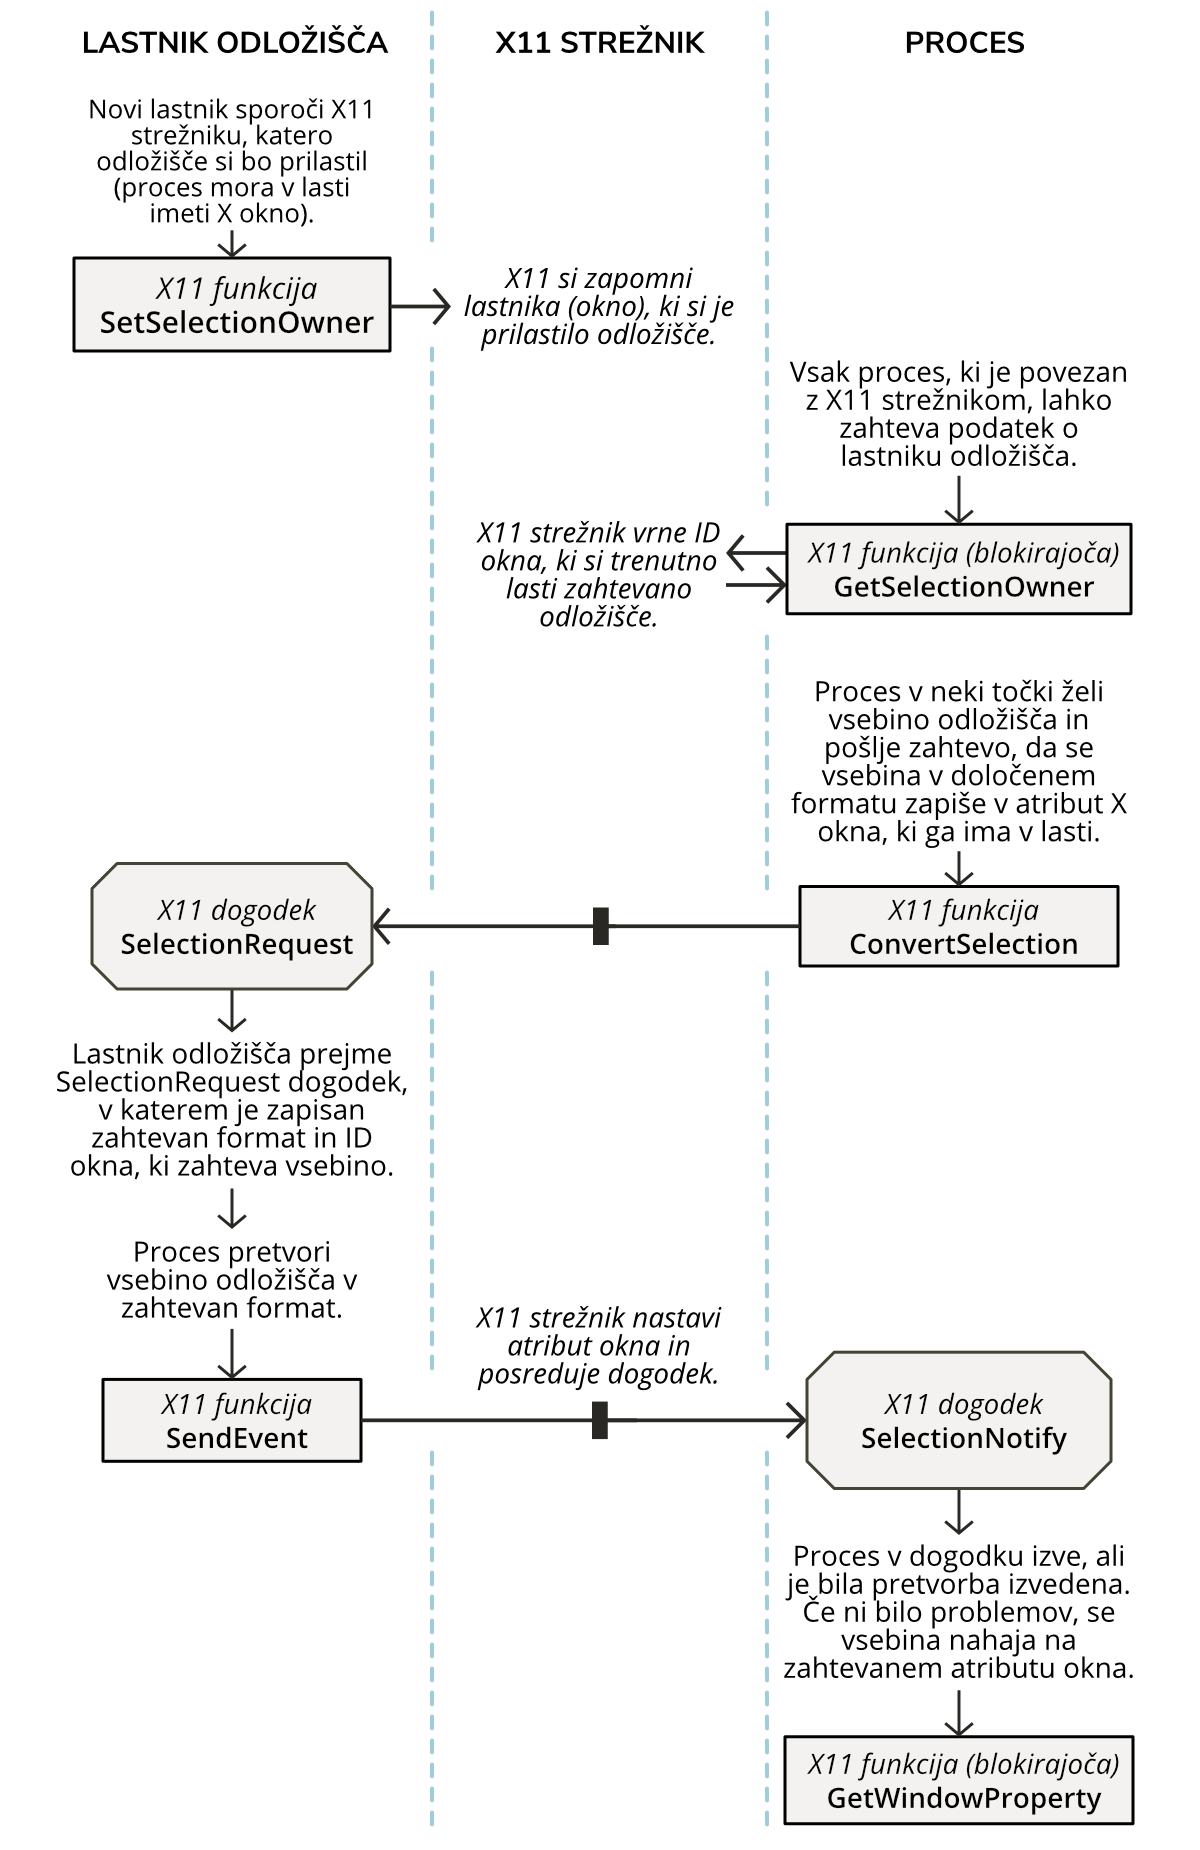
\includegraphics[width=\textwidth]{assets/X11_skica.png}}
	
	
	\subsection{Windows}
	Odložišče na sistemih Windows je malo bolj napredno, a kljub vsemu podobno okenskem sistemu X11 na Linuxu, ki je bilo opisano v prejšnjem poglavju. Ker so koncepti podobni (kot tudi v interesu berljivosti), večine specifičnih funkcij in konstant v tem poglavju ne bom našteval, so pa na voljo v \href{https://docs.microsoft.com/en-us/windows/win32/dataxchg/clipboard-reference}{Microsoftovi dokumentaciji}. \\
	
	Podobno kot pri X11, Windows definira različne formate vsebine v odložišču, ki jih predstavi s pozitivnim celim številom. Aplikacije imajo prav tako možnost registrirati nove formate vsebine. Poleg normalnih operacij ima odložišče še dodaten atribut, ki hrani zaporedno število (ang. "clipboard sequence number"). Ta številka se poveča vsakič, ko se vsebina odložišča spremeni, kar omogoča zaznavo spremembe v odložišču brez dejanske primerjave vsebine.
	
	Vse se začne z "odpiranjem" odložišča. Odpiranje služi kot mehanizem zaklepanja - ko ima določen proces odprto odložišče, vsebine ni mogoče spreminjati. Tega mehanizma na X11 ni.
	
	\textbf{Če želi proces pridobiti lastništvo odložišča}, to stori po odpiranju. V klicu na Win32 API, ki nastavi lastništvo, ima dve možnosti: lahko takoj pošlje dejansko vsebino odložišča (za določen format) ali pa nastavi zastavico, s katero sporoči, da bi vsebino raje izrisal po zahtevi. Tukaj se Windows implementacija razlikuje od Linux specifikacij - X10 je imel sistem z medpomnilnikom, X11 pa zahtevke, med tem ko ima Windows oboje! To poenostavi arhitekturne zahteve majhnih aplikacij, ki bi morale v nasprotnem sistemu podpirati odgovore na zahteve za vsebino odložišča. Obenem pa imajo zahtevnejši uporabniki možnost dinamičnega izrisovanja vsebine.
	
	Na X11 sistemih odložišče postane nedostopno, če se proces konča (ker ne more več odgovarjati na zahteve po vsebini). Na Windows sistemih je dodana majhna podrobnost, ki ta problem odpravi: pred končanjem procesa se sproži še zadnji dogodek imenovan \textit{WM\_RENDERALLFORMATS}, ki od aplikacije zahteva izris vsebine v vseh formatih, ki jih podpira. Nato se proces konča, vsebina pa je kljub temu shranjena!
	
	\textbf{Če želi proces pridobiti vsebino odložišča}, mora najprej preveriti, kateri formati so na voljo. Klic na Win32 API procesu sporoči, kakšne formate podpira lastnik odložišča. Sledi klic, v katerem proces zahteva vsebino v izbranem formatu. Če je lastnik zahteval izrisovanje ob zahtevku, se mu pošlje zahteva za izris.

	Posebnost Windows implementacije je še \textbf{možnost poslušanja sprememb v odložišču}. Vsak proces, ki želi prejemati obvestila, se registrira kot poslušalec. Ko se vsebina odložišča spremeni, proces prejme dogodek \textit{WM\_CLIPBOARDUPDATE}\textsuperscript{\cite{winclipboard}}. Takega sistema na X11 ni.
	
	
	\section{Zaključek}
	V seminarski nalogi sem želel podrobneje raziskati različne pristope odložiščnih sistemov, ki jih uporabljamo zelo pogosto. Ugotovil sem, da imajo implementacije precej skupnih konceptov, a kljub vsemu zaradi različne zgodovine drugačne funkcionalnosti, prednosti in slabosti. V Linux svetu se je začelo s prenašanjem vsebine v centralni proces, ki je hranil vsebino odložišča (X10) in nadaljevalo z opustitvijo prejšnjega sistema in prehoda na bolj kompliciran, a boljši, sistem zahtevkov (X11). Prvi pristop je bil enostavnejši za končne uporabnike, a vsebinsko omejen, drugi pa je za boljšo funkcionalnost plačal z arhitekturno zahtevnostjo aplikacij. V Windows svetu pa imamo na voljo oboje, s čimer pridobimo najboljše lastnosti obeh pristopov.
	
	
	\pagebreak
	\section{Viri}
	\begin{thebibliography}{10}
		\bibitem{winclipboard}
		\textit{Clipboard - Win32 apps | Microsoft Docs.}
		URL: \url{https://docs.microsoft.com/en-us/windows/win32/dataxchg/clipboard}
		
		\bibitem{winclipboardabout}
		\textit{About the Clipboard - Win32 apps | Microsoft Docs.}
		URL: \url{https://docs.microsoft.com/en-us/windows/win32/dataxchg/about-the-clipboard}
		
		\bibitem{xwiki}
		\textit{X Window System - Wikipedia.}
		URL: \url{https://en.wikipedia.org/wiki/X_Window_System}
		
		\bibitem{icccm}
		\textit{ICCCM - Peer-to-Peer Communication by Means of Selections.}
		URL: \url{https://tronche.com/gui/x/icccm/sec-2.html#s-2}
		
		\bibitem{designingiteractions}
		Moggridge, Bill. Designing interactions. Cambridge, Massachusetts: MIT Press, 2007. Strani 64 - 68. ISBN 9780262134743. \\
		(kopija za izposojo na voljo na archive.org: \url{https://archive.org/details/designinginterac00mogg})
		
		\bibitem{xdocs}
		\textit{X Window System Concepts}
		URL: \url{https://www.x.org/wiki/guide/concepts/}
		
		\bibitem{emacsclipboard}
		\textit{X Selections, Cut Buffers, and Kill Rings.}
		URL: \url{https://www.jwz.org/doc/x-cut-and-paste.html}
		
		\bibitem{keithpackardthexselectionmechanism}
		Packard, Keith. The X Selection Mechanism. \url{https://keithp.com/~keithp/talks/}
	\end{thebibliography}
	
\end{document}